\chapter{甜点评价}

\section{任务背景}

甜点评价把地质、储层和生产信息分解为七个具有独立定义的目标。T1 是储层质量指数
代理量 $0.0314\sqrt{\mathrm{KLOGH}/\mathrm{PHIF}}$；T2 是近二元的砂岩标志代理；
T3 是预测时点后 30 个日历日内、至少 24 个有效观测日的平均产油量；T4 是未来
30 日内连续 7 个有效日出现产水的代理标签。T1、T2 和 T4 不是现场甜点真值，
只有 T3 属于观测生产结果。

T5 表示剩余油或加密井潜力，但尚无经审定的标签；T6 和 T7 分别对应解释得到的 PHIF
与 KLOGH，其多模态生产路径尚缺可迁移的开发期地震特征。不同目标的数据量和时间
结构差异很大，因此本赛道按目标选择模型，并分别报告结果。

\section{方法原理}

T1 使用 LightGBM，T2 与 T4 使用 CatBoost。两类提升树都以加法模型逐步拟合残差，
一般形式为
\begin{equation}
  F_t(\bm{x})=F_{t-1}(\bm{x})+\eta f_t(\bm{x}),
\end{equation}
其中 $f_t$ 为第 $t$ 棵树，$\eta$ 为学习率。CatBoost 的有序目标统计有助于降低
类别特征中的目标泄漏。

T3 的主模型为 Chronos-2\cite{ansari2025chronos2}。模型读取目标历史、协变量和
预测时间点，输出未来生产量。为降低短序列上的波动，最终预测与训练期均值进行加权：
\begin{equation}
  \hat{y}_{T3}
  =\alpha\hat{y}_{\mathrm{Chronos2}}
  +(1-\alpha)\bar{y}_{\mathrm{train}},
\end{equation}
其中 $\alpha$ 只在当前训练折内部选择。MOMENT 用于时序表征对照，但不替代已经
通过开发集选择的 T3 路径。

\ArchitectureFigure{sweetspot}
  {甜点评价模型架构。七个目标分别建模，T3 由 Chronos-2 与训练期均值受控融合。}
  {sweetspot-architecture}

\section{训练策略}

静态任务按分组折划分，保证同一井或同一实体不会同时进入训练和验证。时序任务使用
滚动起点验证：每一折只用预测时刻之前的历史训练，并在随后的时间窗验证。T3 每折
最多使用 1024 个训练样本和 512 个验证样本，以固定计算规模。

T3 的融合权重 $\alpha$ 在折内训练数据上选择，再应用于该折验证窗口。候选模型按
平均绝对误差排序。T4 属于类别不平衡任务，因此按平均精确率选择，而不是按准确率
选择。T5--T7 在数据或任务定义不足时不训练占位模型。

\TrainingFlow
  {七项目标与协变量}
  {分组或滚动划分}
  {目标专属模型训练}
  {折内参数选择}
  {逐目标独立评价}
  {甜点评价训练流程}
  {sweetspot-training}

\section{实验设计}

T1 和 T2 的输入为静态井曲线，输出分别为 RQI 代理量与砂岩标志。T3 的输入为截止
$t_0$ 的产油、产气、产水、开井时长、井底压力、节流阀与井口压力序列，输出
$t_0+1$ 至 $t_0+30$ 日的平均产油量。T4 使用同类历史序列预测 30 日产水事件。
不完整时间窗作删失处理，不把缺测日填成零。

T3 同时比较三个基准：训练历史均值、归档 XGBoost 和 Chronos-2 融合。T4 比较
CatBoost 与 Chronos 候选分支。开发样本量分别为 T1 35810、T2 36122、T3 1111
和 T4 32；已知留出样本量分别为 11936、12081、132 和 37。T5 当前不可行，
T6 与 T7 仍受输入数据限制。

\section{评估指标}

回归任务使用 MAE、RMSE 和 $R^2$。其中
\begin{equation}
  \Metric{MAE}=\frac{1}{N}\sum_i|y_i-\hat{y}_i|,
  \qquad
  \Metric{RMSE}=\sqrt{\frac{1}{N}\sum_i(y_i-\hat{y}_i)^2}.
\end{equation}
分类任务使用平均精确率、Macro-F1 和 ROC-AUC。平均精确率对精确率--召回率曲线
进行加权求和：
\begin{equation}
  \Metric{AP}=\sum_n(R_n-R_{n-1})P_n,
\end{equation}
其中 $P_n$ 和 $R_n$ 分别为第 $n$ 个阈值下的精确率和召回率。每个目标独立评价，
不把不同单位的指标相加为综合分数。

\section{实验结果}

\begin{table}[htbp]
  \centering
  \caption{T3 时序预测的滚动验证结果}
  \label{tab:sweetspot-t3-dev}
  \begin{tabular}{lrr}
    \toprule
    模型 & MAE & 相对 Chronos-2 的 MAE 增幅 \\
    \midrule
    归档 XGBoost & 267.1180 & $+43.17\%$ \\
    因果历史均值 & 204.6371 & $+9.68\%$ \\
    Chronos-2 融合 & \textbf{186.5715} & -- \\
    \bottomrule
  \end{tabular}
\end{table}

\Cref{tab:sweetspot-t3-dev}显示，Chronos-2 融合的 MAE 为 $186.57$，相对归档
XGBoost 降低 $30.15\%$，相对
因果历史均值降低 $8.83\%$，满足预设的开发集改进标准。T4 中，Chronos 分支的
AP 为 $0.5091$，低于 CatBoost 的 $0.6541$，因此未达到改进标准。两项结果说明同一基础模型
在不同目标上可能产生相反结论，必须逐任务评价。

\begin{table}[htbp]
  \centering
  \caption{四个可评价目标的已知留出结果}
  \label{tab:sweetspot-holdout}
  \small
  \begin{tabular}{llllr}
    \toprule
    目标 & 留出模型 & 主要指标 & 辅助指标 & 样本量 \\
    \midrule
    T1 & LightGBM & $R^2=0.8968$ & MAE $=0.2162$ & 11936 \\
    T2 & CatBoost & AP $=0.9991$ & F1 $=0.9777$ & 12081 \\
    T3 & 归档 XGBoost & MAE $=47.7020$ & $R^2=-0.0636$ & 132 \\
    T4 & CatBoost & AP $=0.1315$ & F1 $=0.1951$ & 37 \\
    \bottomrule
  \end{tabular}
\end{table}

\Cref{tab:sweetspot-holdout}报告的是早期阶段固定模型在已知留出集上的确认结果，
不能解释为 Chronos-2 的留出表现。尤其是 T4 的开发 AP 为 $0.6541$，已知留出
AP 仅为 $0.1315$；结合留出样本量只有 37，这一差异提示小样本波动和分布偏移风险。

\ResultFigure{0.98}{sweetspot}{research_target_diagnostics.png}
  {T1 储层质量代理的逐深度观测、预测与残差，以及 T3 生产率在因果时间轴上的观测、
  预测与残差。两个目标保持独立单位，不合成为单一评分。}

\ResultFigure{0.92}{sweetspot}{research_productivity_performance.png}
  {T3 已知留出集的实测--预测散点与标准化残差 Q--Q 图。散点按预测时序着色，
  虚线分别表示理想预测和正态残差参照。}

T3 的确认模型在已知留出集上取得 $R^2=-0.0636$，实测--预测散点仍明显偏离
单位线。残差 Q--Q 图在两端偏离参照线，说明极端生产阶段的误差不能由简单正态扰动
解释。该结果与开发阶段的 Chronos-2 改进并不矛盾：两者对应不同模型和证据阶段，
真正的下一步是对 Chronos-2 完成同口径时序留出评价，而不是用开发增益替代留出结论。

\ResultFigure{0.96}{sweetspot}{overview_seven_targets.png}
  {甜点评价七个目标的定义、数据可用性与主要结果总览。}

\ResultPair{sweetspot}
  {T1_regression_diagnostics.png}{T1 回归诊断}
  {T2_classification_diagnostics.png}{T2 分类诊断}
  {T1 与 T2 的实验结果}

\ResultPair{sweetspot}
  {T3_regression_diagnostics.png}{T3 时序回归诊断}
  {T4_classification_diagnostics.png}{T4 分类诊断}
  {T3 与 T4 的实验结果}

\begin{figure}[htbp]
  \centering
  \begin{subfigure}[t]{0.32\textwidth}
    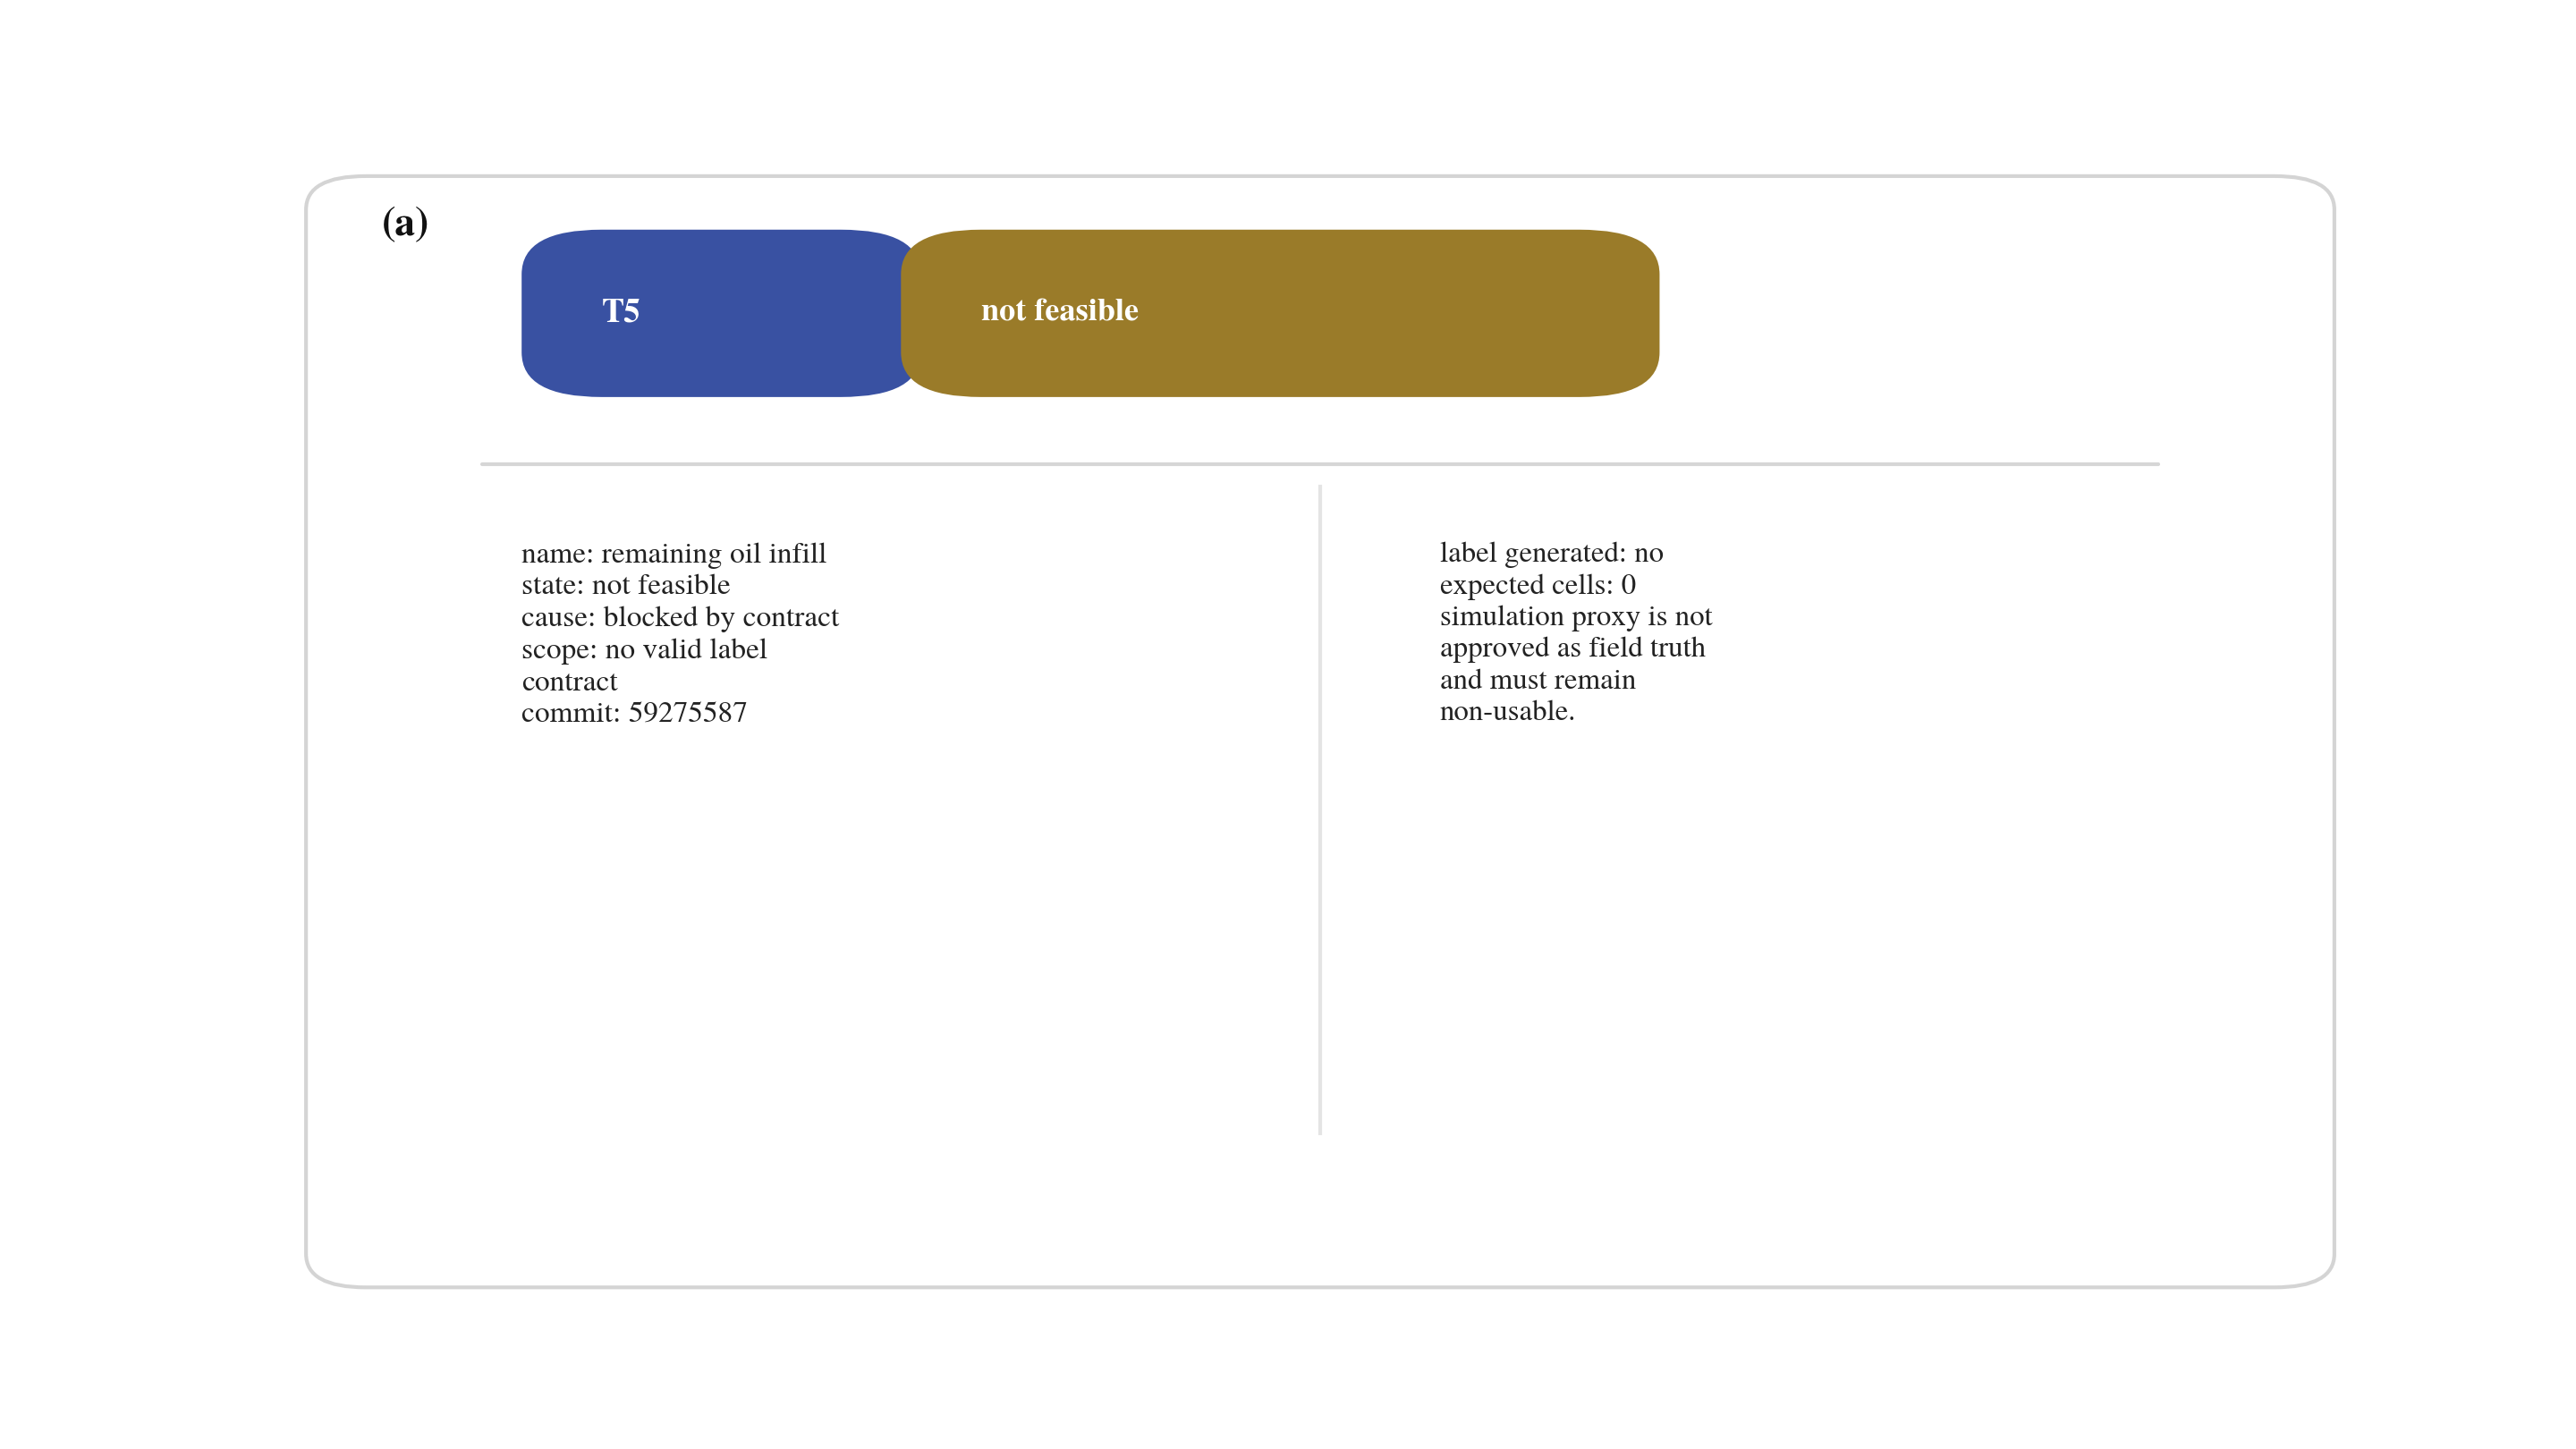
\includegraphics[width=\textwidth]{../figures/results/sweetspot/T5_status_card.png}
    \caption{T5}
  \end{subfigure}\hfill
  \begin{subfigure}[t]{0.32\textwidth}
    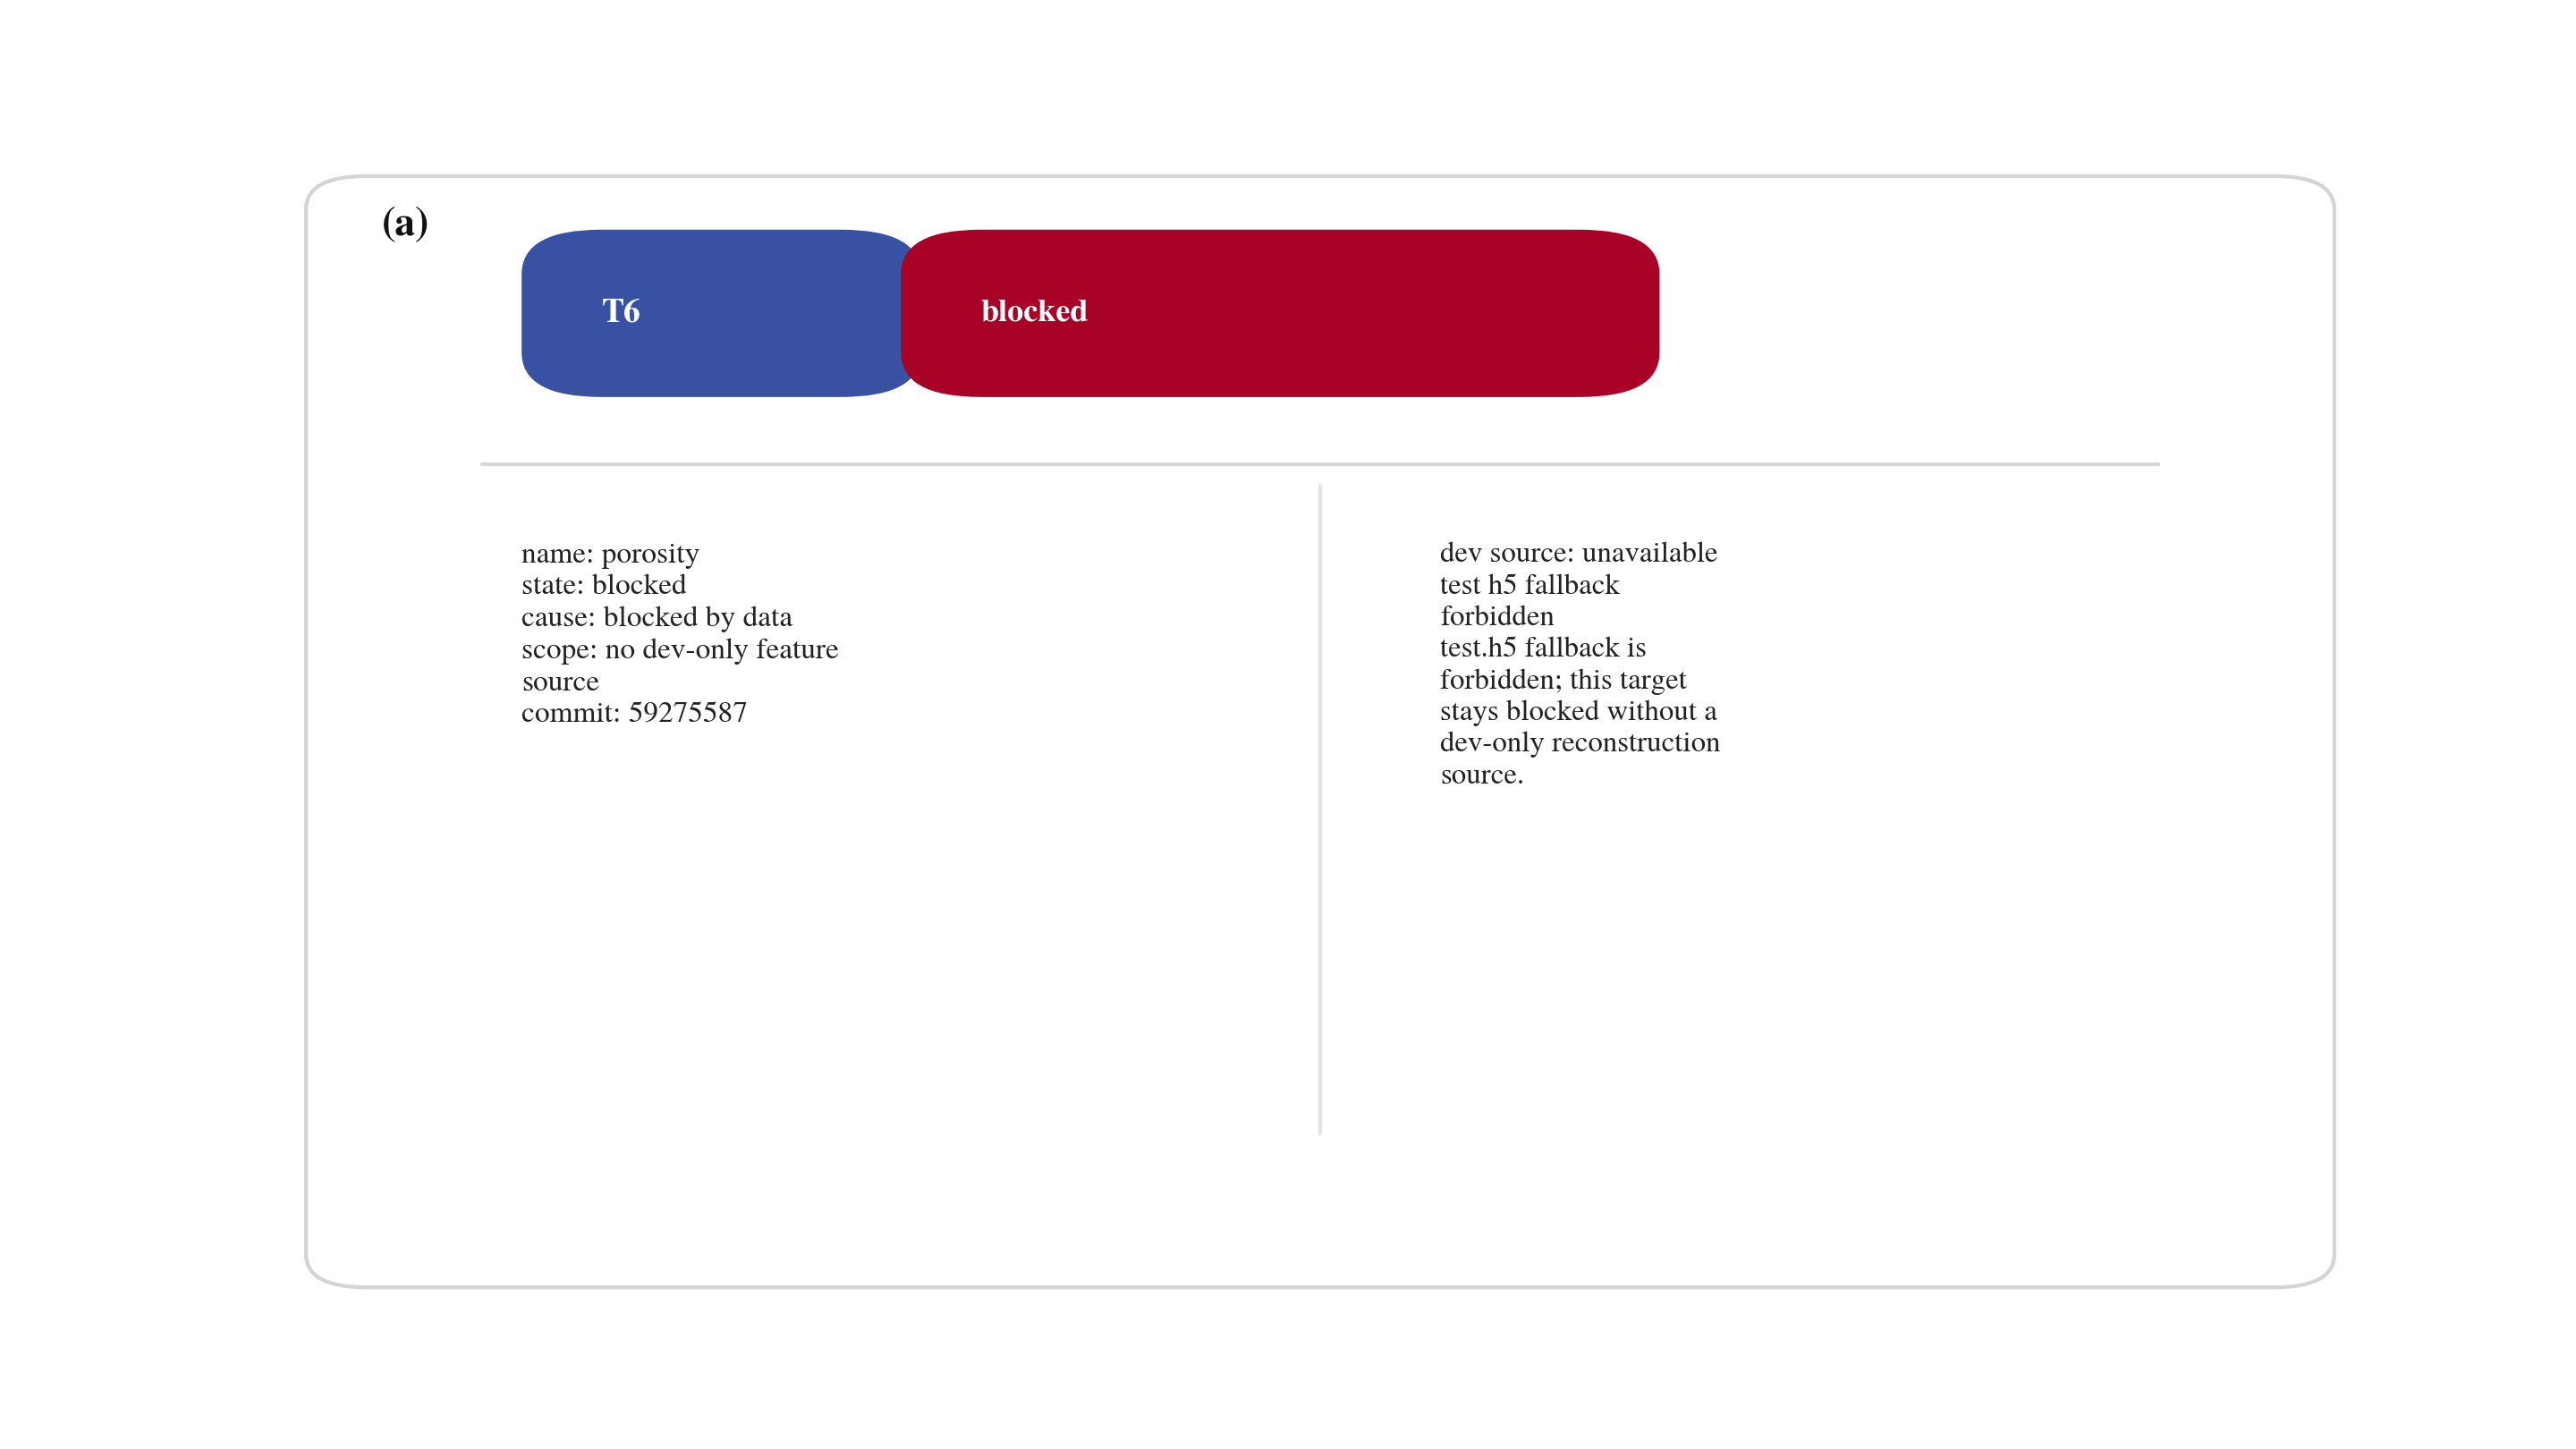
\includegraphics[width=\textwidth]{../figures/results/sweetspot/T6_status_card.png}
    \caption{T6}
  \end{subfigure}\hfill
  \begin{subfigure}[t]{0.32\textwidth}
    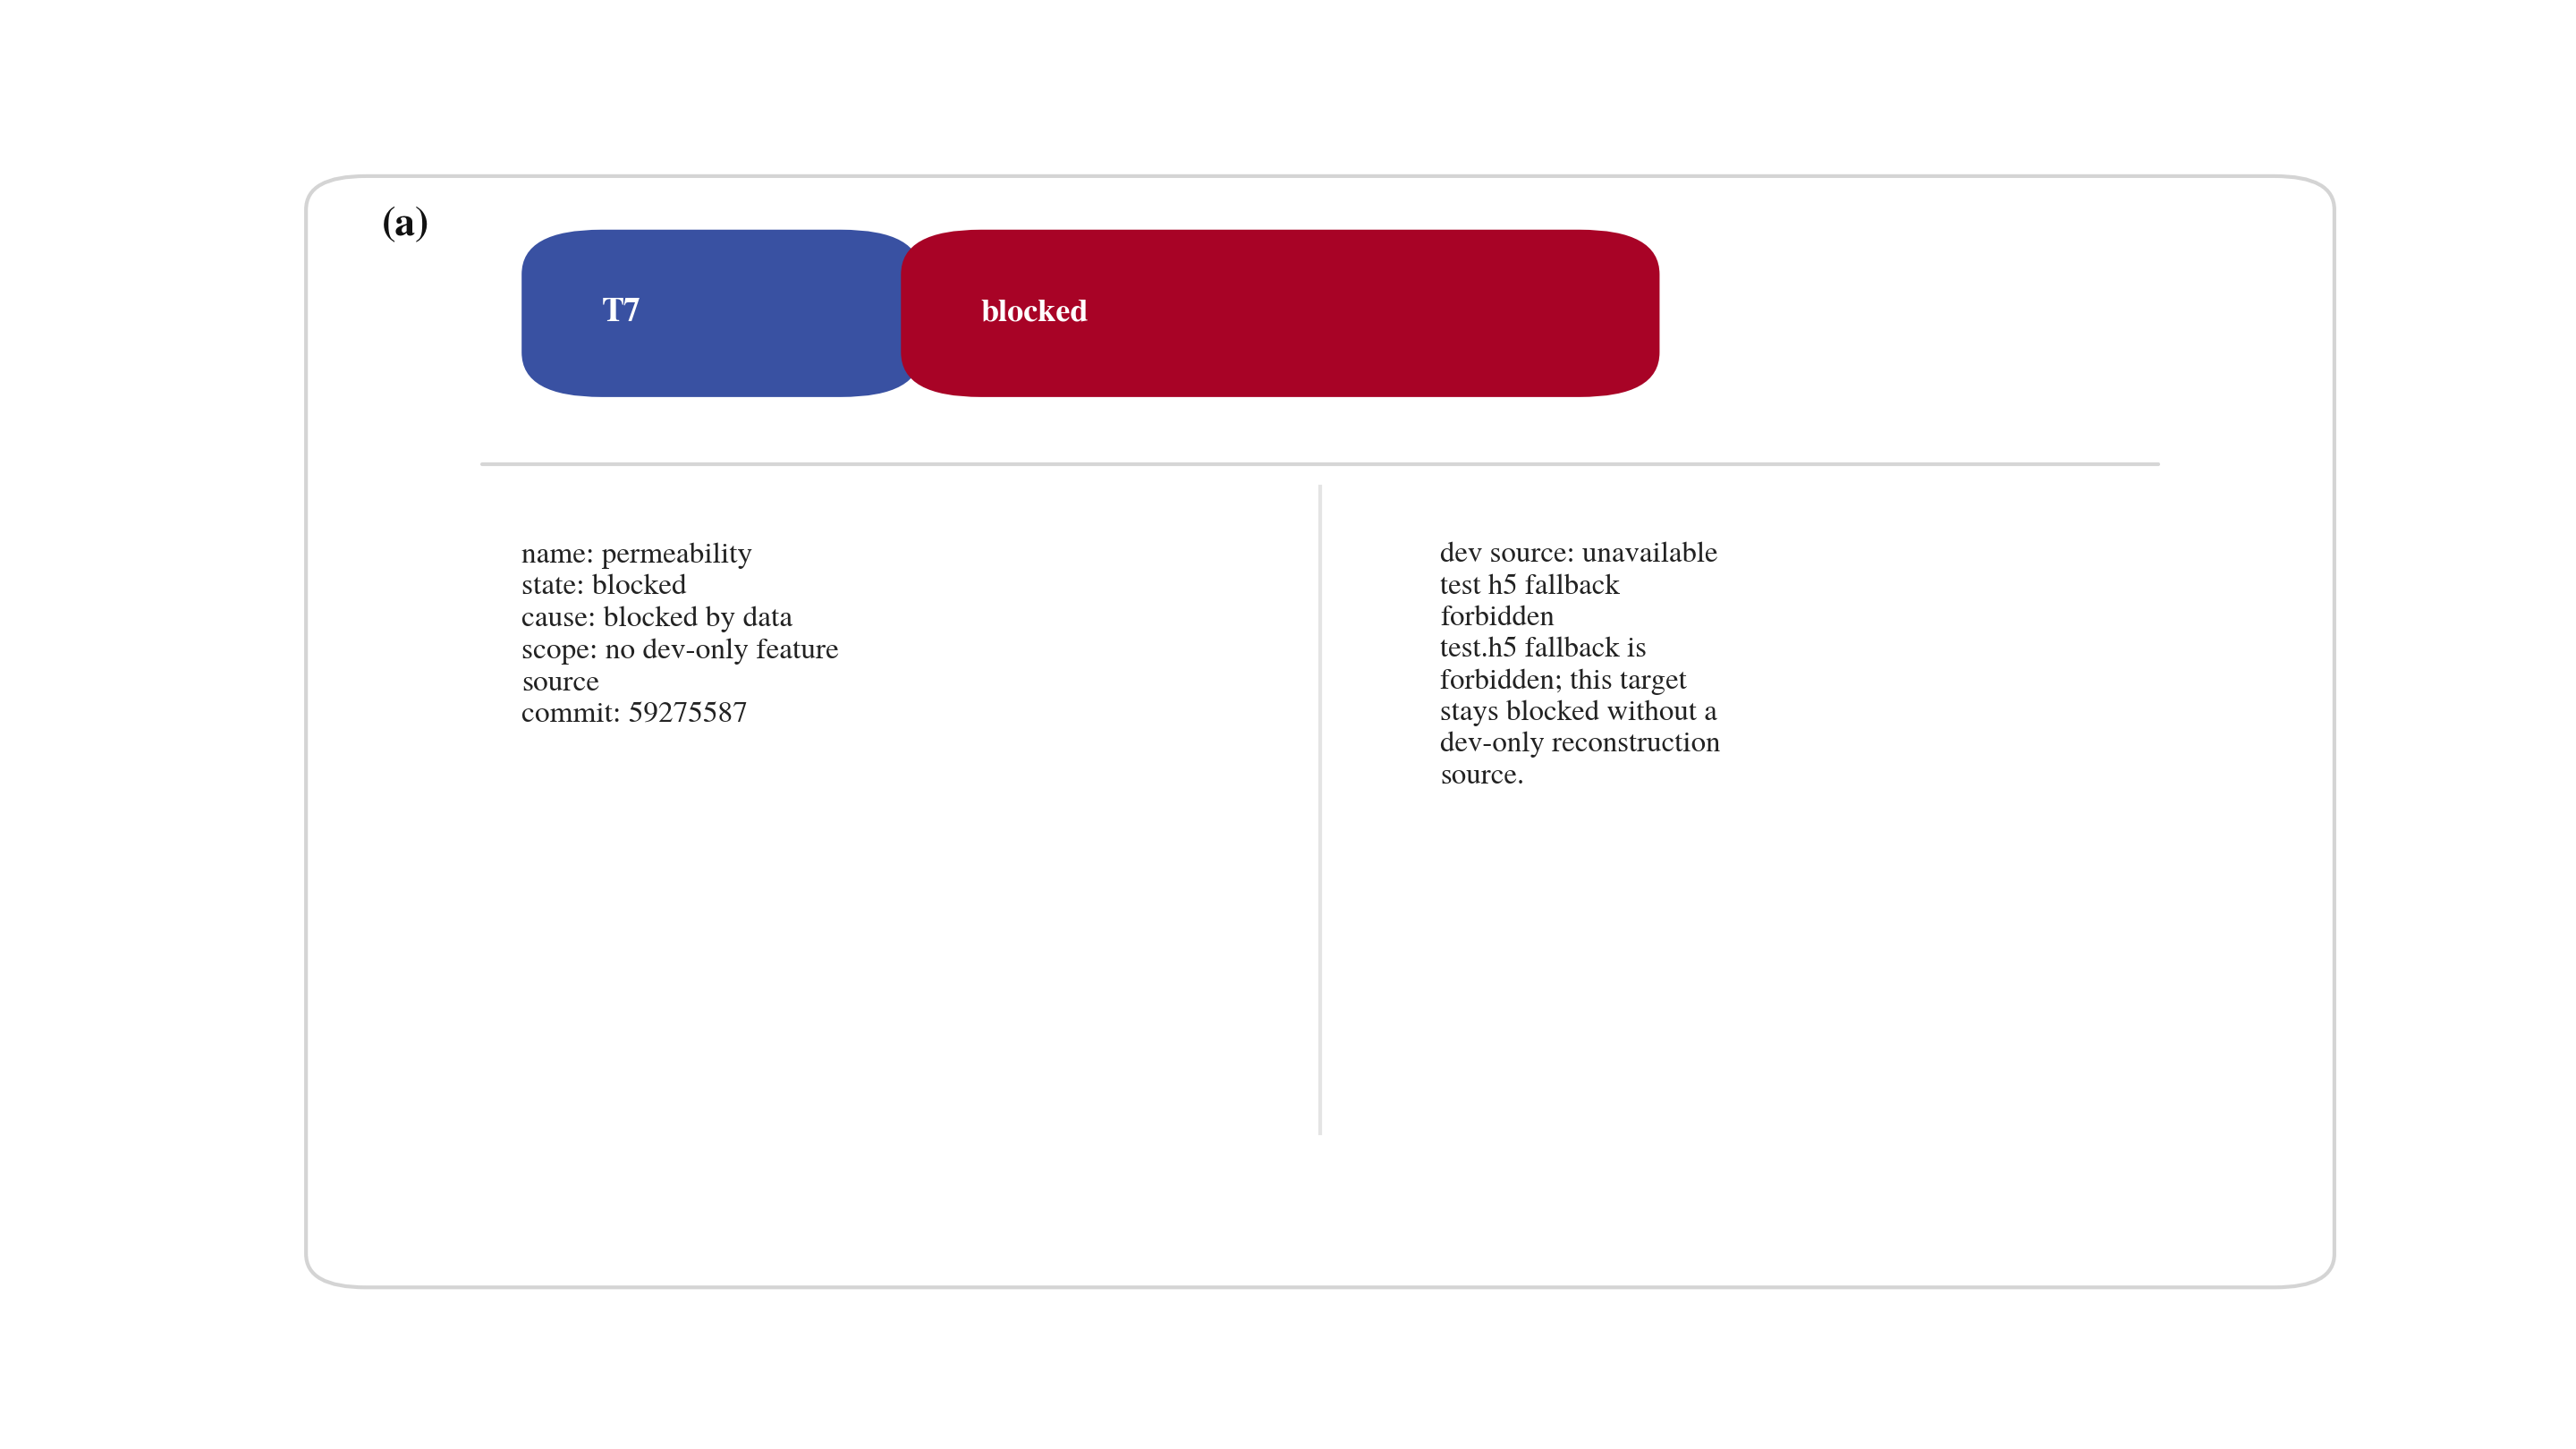
\includegraphics[width=\textwidth]{../figures/results/sweetspot/T7_status_card.png}
    \caption{T7}
  \end{subfigure}
  \caption{T5--T7 的数据可用性。T5 缺少经审定标签，T6--T7 缺少完整多模态开发输入。}
\end{figure}

本次基础模型实验中，明确的开发集改进来自 T3。T1、T2 和 T4 已完成固定模型评价；
T5--T7 在标签或输入不完整时不构造替代结果。逐目标报告避免把不同物理含义和单位的
指标合并为一个表面精确、实际难以解释的综合分数。

\FloatBarrier
